\documentclass[11pt,a4paper]{article}
\usepackage[utf8]{inputenc}
\usepackage[hmargin=2.0cm,vmargin=2.5cm,bindingoffset=0.5cm]{geometry}
\usepackage{amsfonts}
\usepackage{amsmath,amsthm,amssymb}
\allowdisplaybreaks
\usepackage{hyperref}
\usepackage{graphicx}
\usepackage{tikz}
\usepackage{mathtools}
\DeclarePairedDelimiter\ceil{\lceil}{\rceil}
\DeclarePairedDelimiter\floor{\lfloor}{\rfloor}
%\usepackage{float}
\usepackage{placeins}
\usepackage{diagbox}
\DeclareMathOperator{\Tr}{Tr}
\newtheorem{thm}{Theorem}
\usepackage{subcaption}
%\usepackage{subfigure}
\usepackage[english]{babel}
\author{Mohit}
\title{Quantum control of NV center using counter-diabatic driving  }
\begin{document}
\maketitle
%\tableofcontents

\section{Introduction}
 The Hamiltonian for the ground state of the NV center can be written as :
\begin{equation}
H_{NV}= \hbar \Delta S_z^2 + \hbar \gamma_e \vec{S}. \vec{B}_{ext} +  \hbar \gamma_n \vec{I}. \vec{B}_{ext} + A \vec{S}. \vec{I}
\end{equation}
where $\Delta= 2 \pi \times 2.87 $ GHz is zero-field splitting, $\gamma_e =2.8 MHz/G$ is the gyromagnetic ratio of electron in the NV center, $\gamma_n \simeq 1 kHz/G$ is the gyromagnetic ratio of nuclear spin, $\vec{S}$ ($\vec{I}$ ) is the spin of electron (nucleus) and $A \simeq 3 MHz$ is magnitude of spin-spin coupling which leads to hyperfine splitting. The second and third terms are due to Zeeman effect.

Since $\gamma \propto 1/m$ and nucleus is heavier than electron, we have $\gamma_e \gg \gamma_n$. To simplify our model, we will ignore the last two terms resulting in the following Hamiltonian :
\begin{equation}
H_{NV}= \hbar \Delta S_z^2 + \hbar \gamma_e \vec{S}. \vec{B}_{ext} 
\end{equation}
It seems that the above Hamiltonian should be experimentally realizable \cite{dhingra2017nitrogen}. Moreover, the ground state of electron in the NV center is a spin triplet with $| 0 \rangle, | -1 \rangle, | 1 \rangle$ spin sub-levels. They are defined in $S_z$ basis , where $\hat{z}$ direction is along the NV center axis. If there is no external magnetic field, then $| -1 \rangle$ and $| 1 \rangle$ levels are degenerate, and  $ \hbar \Delta$ is the energy difference between $| 0 \rangle$ and $| \pm 1 \rangle$ energy levels.

\section{Static magnetic field}

Let's choose magnetic field to be in x-direction \footnote{If magnetic field is in z-direction, then gauge potential is zero. This is so because increasing $B_z$ does not induce any excitations. }. Then we have:
\begin{align*}
H_{NV} &= \hbar \Delta S_z^2 + \hbar \gamma_e   S_x  B = \Lambda S_z^2 + \lambda   S_x  
\end{align*}
where $\Lambda= \hbar \Delta $ and $\lambda=\hbar \gamma_e B $. Magnetic field is going to be our control parameter in this problem. 

\subsection{Energy levels as a function of magnetic field}

Using spin algebra  (appendix \ref{sec.spin_alegbra}), we obtain Hamiltonian in the $S_z$ basis ($|- 1\rangle$, $| 0 \rangle$ , $| 1 \rangle$):

\begin{equation}
H= \begin{pmatrix}
    \beta       & \alpha  & 0  \\
    \alpha       & 0 &\alpha  \\
     0       & \alpha & \beta
\end{pmatrix}
\quad \mbox{where}  ~
 \alpha= \lambda/ \sqrt{2}, ~ \beta=  \Lambda
\end{equation}


\begin{figure}[!ht]
\begin{center}
\includegraphics[scale=0.5]{pics/energy_level_beta1.eps} 
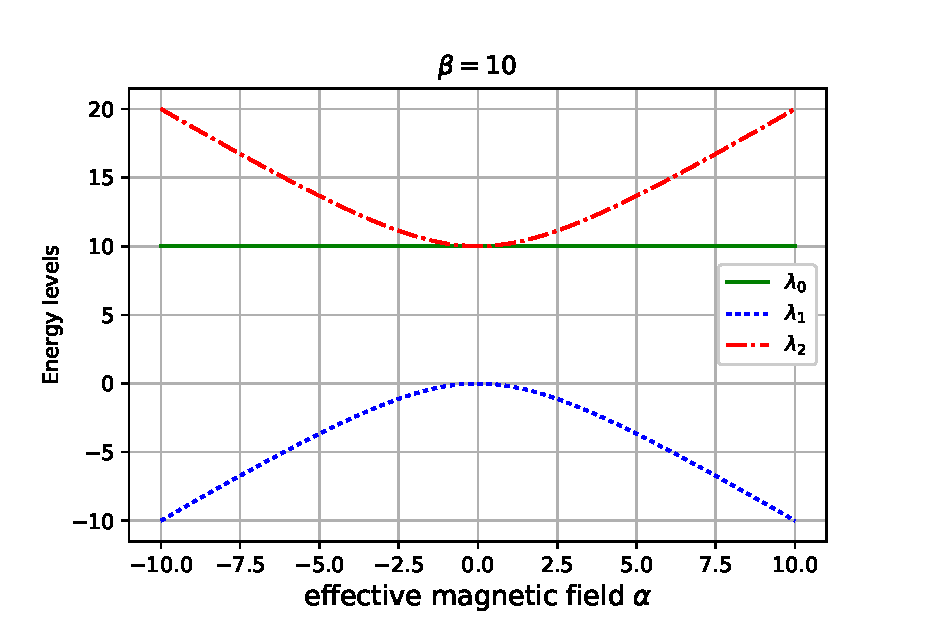
\includegraphics[scale=0.5]{pics/energy_level_beta10.eps} 
\caption{Avoided level crossing as a function of effective magnetic field }
\label{ev}
\end{center}
\end{figure}

 Energy eigenvalues are given by:
\begin{align*}
\lambda_0 &= \beta, \quad \lambda_1 = (\beta - \sqrt{\beta^2 + 8 \alpha^2})/2 , \quad  \lambda_2 = (\beta + \sqrt{\beta^2 + 8 \alpha^2})/2
\end{align*}
We should remember that $\alpha \propto B$. Hence, it makes sense that when $\alpha=0$,  there is a two -fold degeneracy and zero field energy gap is given by $\beta=\hbar \Delta$. Now let's have a look at eigenvectors:
\begin{align*}
\nu_0 = (-1,0,1), \quad \nu_1 = (1, -(\beta + \sqrt{\beta^2 + 8 \alpha^2})/2 \alpha, 1) , \quad \nu_2 = (1, -(\beta - \sqrt{\beta^2 + 8 \alpha^2})/2 \alpha, 1)
\end{align*}

\subsection{Adiabatic gauge potential}

Now let's compute adiabatic gauge potential $A_{\lambda}= i \hbar \partial_{\lambda}$. Its' equation of motion is given by:
\begin{equation}
[H, \partial_{\lambda} H +\dfrac{i}{\hbar} [A_{\lambda}, H] ]=0
\label{eom}
\end{equation}

Eigen-value equation is given by $H (\lambda) |n(\lambda) \rangle = E_n (\lambda) |n(\lambda) $. Let's derive diagonal and off-diagonal elements:

\begin{itemize}
\item \textbf{n-th diagonal element:} $A_{\lambda}^n= \langle n |A_{\lambda} | n \rangle=  i \hbar\langle n |\partial_{\lambda} | n \rangle $

%Now since $\alpha= \hbar \lambda/ \sqrt{2} $, we have $\partial_{\lambda}=  \frac{d \alpha}{d \lambda}\partial_{\alpha} =\frac{\hbar}{\sqrt{2}} \partial_{\alpha}$.
%
% Now let's have a look at eigenvectors:
%\begin{align*}
%| n=0 \rangle = \begin{bmatrix}
%-1 \\
%0 \\
%1
%\end{bmatrix}, \quad | n=1 \rangle = \begin{bmatrix}
%1 \\
%\nu_1 \\
%1 
%\end{bmatrix}
%, \quad 
%| n=2 \rangle = \begin{bmatrix}
%1 \\
%\nu_2 \\
%1 
%\end{bmatrix}
%\end{align*}
%where $\nu_1= -(\beta + \sqrt{\beta^2 + 8 \alpha^2})/2 \alpha $ and $\nu_2=-(\beta - \sqrt{\beta^2 + 8 \alpha^2})/2 \alpha$.
%
%Hence, $A_{\lambda}^{n=0}= 0$
\item \textbf{off- diagonal element:} We use the identity $\langle m |H(\lambda) | n \rangle=0 \quad, n \neq m$ and then differentiate with respect to $\lambda$ to obtain:
\begin{align}
\langle m |A_{\lambda} | n \rangle =  -i \hbar \dfrac{\langle m |\partial_{\lambda}H | n \rangle}{E_m-E_n}
\end{align}
where both  energies ($E_m, E_n$) and eigenvectors ($|m \rangle, |n \rangle$) depend on $\lambda$.
\end{itemize}


Here $\partial_{\lambda} H=S_x$ whose matrix representation is given in appendix \ref{sec.spin_alegbra}. We find that $\tilde{A_{\lambda}} $ in energy basis is given by :

\begin{equation}
\tilde{A_{\lambda}}=i\hbar \tilde{N}
\begin{pmatrix}
0 & 0 & 0\\
0 & 0 & -1 \\
0 & 1 & 0
\end{pmatrix}, \quad \mbox{where} ~ \tilde{N} =\dfrac{ \beta \hbar}{8 \alpha^{2} + \beta^{2}}
\end{equation}


In $S_z$ basis, we have  $A_{\lambda}= U\tilde{A_{\lambda}} U^{T}$ where $U$ is the unitary transformation that diagonalizes Hamiltonian, i.e. $H_d= U^THU$. $A_{\lambda}$ is given below:

\begin{align*}
A_{\lambda}=i\hbar N
\begin{pmatrix}
0 & -1 & 0\\
1 & 0 & 1 \\
0 & -1 & 0
\end{pmatrix}, \quad \mbox{where} ~ N =\dfrac{ \beta \hbar}{\sqrt{16 \alpha^{2} + 2\beta^{2}}}
\end{align*}


%\end{equation}



The above matrix of $A_{\lambda}$ can be expanded in the basis of $SU(3)$ to expand. This basis is composed of Gell–Mann matrices \cite{gell1962symmetries}, which are represented as $\lambda_i$. For our purpose, most important Gell-Mann matrices are $\lambda_2$ and $\lambda_7$ whose representation is given below \cite{ bertlmann2008bloch, krammer2009entanglement}:

\begin{align*}
\lambda_2 = \begin{pmatrix} 0 & -i & 0 \\ i & 0 & 0 \\ 0 & 0 & 0 \end{pmatrix} 
= \dfrac{1}{\sqrt{2} \hbar^2}(\hbar S_y+ S_y S_z+  S_z S_y)\\
\lambda_7= \begin{pmatrix} 0 & 0 & 0\\0 & 0 & -i \\0 & i & 0\end{pmatrix}= \dfrac{1}{\sqrt{2} \hbar^2}(\hbar S_y- S_y S_z-  S_z S_y)
\end{align*}

Hence, we find that $A_{\lambda}=\hbar N(\lambda_2- \lambda_7)$ which can be written as:

\begin{equation}
\boxed{
A_{\lambda}=N_0(S_y S_z+  S_z S_y)}
\end{equation}
where $N_0 =\dfrac{ \beta }{\sqrt{8 \alpha^{2} + \beta^{2}}}= \dfrac{ \Delta }{ \sqrt{4  \gamma_e^2 B^2 + \Delta^2}}$.



 
\section{Periodic magnetic field with noise}

Let's choose magnetic field to be $\vec{B}= (B_x (t), 0, 0)$ where $B_x(t)= B_0 \sin (\omega t) + \epsilon(t)$ and  $\epsilon(t)$ is an infinitesimal white noise which satisfies $\overline{ \epsilon(t) \epsilon(t^{\prime})}= \kappa \delta(t -t^{\prime})$ \footnote{If the system is in equilibrium, then fluctuation -dissipation theorem dictates $\kappa = T$}. 

Then we have: 
\begin{align*}
H_{NV} &= \Lambda S_z^2 + \hbar \gamma_e   S_x  B_x(t) \\
 &=  \Lambda S_z^2 + \lambda   S_x  
\end{align*}
where $\Lambda= \hbar \Delta $ and $\lambda=\hbar \gamma_e (B_0 \sin (\omega t) + \epsilon(t))$. For now on, we will work in the unit in which $\hbar \gamma_e =1$ so that  $\lambda= (B_0 \sin (\omega t) + \epsilon(t))$ and $\Lambda=  \Delta / \gamma_e $.

Using Fermi Golden rule, we can derive transition rate $\langle \Gamma_n \rangle$ \cite{kolodrubetz2016geometry} as follows: 
\begin{align}
 \Gamma_n (\omega) = \kappa  \sum_{m \neq n} |\langle n | G_{\lambda} | m \rangle |^2 \delta(E_n-E_m- \hbar \omega)
\end{align}
where $G_{\lambda}= \partial_{\lambda} H + \dfrac{i}{\hbar} [A_{\lambda}, H]$ and  $\omega$ is frequency of the periodic external drive. More details are given in appendix.


\appendix
\section{Gell-Mann matrices}
\begin{align*}
\lambda_1 &= \begin{pmatrix} 0 & 1 & 0 \\ 1 & 0 & 0 \\ 0 & 0 & 0 \end{pmatrix}
\quad \lambda_2 = \begin{pmatrix} 0 & -i & 0 \\ i & 0 & 0 \\ 0 & 0 & 0 \end{pmatrix}
\quad \lambda_3 = \begin{pmatrix} 1 & 0 & 0 \\ 0 & -1 & 0 \\ 0 & 0 & 0 \end{pmatrix}\\
\lambda_4 &= \begin{pmatrix} 0 & 0 & 1 \\ 0 & 0 & 0 \\ 1 & 0 & 0 \end{pmatrix} \quad
\lambda_5 = \begin{pmatrix} 0 & 0 & -i \\ 0 & 0 & 0 \\ i & 0 & 0 \end{pmatrix} \quad
\lambda_6 = \begin{pmatrix} 0 & 0 & 0 \\ 0 & 0 & 1 \\ 0 & 1 & 0 \end{pmatrix} \\
\lambda_7 &= \begin{pmatrix} 0 & 0 & 0 \\ 0 & 0 & -i \\ 0 & i & 0 \end{pmatrix} \quad
\lambda_8 = \frac{1}{\sqrt{3}} \begin{pmatrix} 1 & 0 & 0 \\ 0 & 1 & 0 \\ 0 & 0 & -2 \end{pmatrix}
\end{align*}
These matrices are traceless and Hermitian.

\section{Spin Algebra}\label{sec.spin_alegbra}
\begin{equation}
[S_x, S_y]=i \hbar S_z, \quad [S_y, S_z]=i \hbar S_x \quad [S_z, S_x]=i \hbar S_y
\end{equation}
\begin{equation}
S^2|s ,m \rangle = \hbar^2 s(s+1)|s ,m\pm 1\rangle  \quad S_z|s ,m \rangle = \hbar m |s ,m \rangle
\end{equation}
\begin{equation}
S_{\pm}|s, m\rangle = \hbar\sqrt{s(s+1)-m(m \pm 1)}|s,m \pm 1\rangle
\end{equation}
where $S_+ = S_x + iS_y$ and $S_- = S_x - iS_y $. Hence, we get $S_x = (S_+ + S_-)/2$ and $S_y = (S_+ - S_-)/2i $
\begin{equation}
S_+= \sqrt{2} \hbar\begin{pmatrix}
0 & 1 & 0\\
0 & 0 & 1\\
0 & 0 & 0\\
\end{pmatrix}
\quad
S_-=\sqrt{2} \hbar 
\begin{pmatrix}
0 & 0 & 0\\
1 & 0 & 0\\
0 & 1 & 0\\
\end{pmatrix}
\end{equation}
Hence, \begin{equation}
S_x= \frac{\hbar}{\sqrt{2} }
\begin{pmatrix}
0 & 1 & 0\\
1 & 0 & 1\\
0 & 1 & 0\\
\end{pmatrix} \quad
S_y=  i \frac{\hbar}{\sqrt{2} }
\begin{pmatrix}
0 & -1 & 0\\
1 & 0 & -1\\
0 & 1 & 0\\
\end{pmatrix}
\end{equation}



\section{Transition rate for periodically driven noisy system}
Let's consider a Hamiltonian:
\begin{equation}
\mathcal{H}_{\mathcal{X}} = \mathcal{H} (\lambda) + \dot{\lambda} \mathcal{X}
\end{equation}
where $\lambda= \lambda_0 + \epsilon(t)$ and  $\epsilon(t)$  is an infinitesimal white noise which satisfies $\overline{ \epsilon(t) \epsilon(t^{\prime})}= \kappa \delta(t -t^{\prime})$ \footnote{If the system is in equilibrium, then fluctuation -dissipation theorem dictates $\kappa = T$}. 
A system under white noise would lead to transitions between all eigenstates. We will see how much there is reduction in transition and dissipation rate with our approximate gauge potential.

We can simplify the above expression:
\begin{equation}
\mathcal{H}_{\mathcal{X}} \approx \mathcal{H} (\lambda_0)+ \epsilon \partial_{\lambda}\mathcal{H} + \dot{\epsilon} \mathcal{X}
\end{equation}
Our expressions will involve $G_{\lambda}$ which is given as $G_{\lambda}(\mathcal{X} )= \partial_{\lambda} H + \dfrac{i}{\hbar} [\mathcal{X}, H] $ where $\mathcal{X}=A_{\lambda}$.


Now we would drive the system periodically in addition to the white noise we have in the system. So, in this protocol, time dependence of $\lambda$ is given as $\lambda(t)= \lambda_0 \sin (\omega t) + \epsilon(t)$. We can use Fermi's golden rule (using results from \cite{clerk2010introduction}) to derive  transition rate $\langle \Gamma_n \rangle$ \cite{kolodrubetz2016geometry} as follows: 
\begin{align}
 \Gamma_n (\omega) = \kappa  \sum_{m \neq n} |\langle n | G_{\lambda} | m \rangle |^2 \delta(E_n-E_m- \hbar \omega)
\end{align}
where $\omega$ is frequency of the periodic external drive.

%
%\section{Gauge potential: expression involving commutators}\label{sec.potn}
%
%Another way to express the formula of adiabatic gauge potential:
%\begin{equation}
% A_{\lambda}(\mu) =  -i\hbar \lim_{\mu \rightarrow 0} \sum_{n=0}^{\infty}   (-1)^{n} \dfrac{ C^{(2n+1)}}{\mu^{2n+2}}
%\end{equation}
%where $C^{(n)}$ is n- commutator of $H$ and $\partial_{\lambda} H$, i.e. $C^{(n)}= [H, [H, \mbox{ n times} \ldots,[H, \partial_{\lambda} H ]]] ] $.  We define the first term as $C^{(1)}= [H, \partial_{\lambda}H]$, second term as $C^{(2)}= [H,[H, \partial_{\lambda}H]]= [H, C^{(1)}]$ and so on and forth.
%
%Let's find out $A_{\lambda}$ for this Hamiltonian for which we need to compute different odd-powered commutator $[H, \partial_{\lambda} H]$, where $\partial_{\lambda} H=S_x$. It turns out that I am not able to compute the summation as the expressions of commutators is pretty involved (details are given in appendix \ref{sec.potn}). I would need to think of some smarter way to compute adiabatic gauge potential.
%
%Here we begin:
%\begin{align*}
%C^{(1)}=[H,S_x] &= \Lambda  [S_z^2, S_x] \\
%&= S_z[S_z, S_x] + [S_z, S_x] S_z \\
%&= i \hbar (S_z S_y + S_y S_z) \\
%&=i \hbar ([S_z, S_y] +  2 S_y S_z)\\
%&=i \hbar (- i \hbar S_x +  2 S_y S_z)
%\end{align*}
%
%\begin{align*}
%C^{(2)}=[H,C^{(1)}] &=     \hbar^2 [H,  S_x]  +  i \hbar[ H,   S_y S_z] \\
%&= \hbar^2 C^{(1)}  +  i \hbar S_y[ H,    S_z] +  i \hbar[ H,   S_y ]S_z\\
%&= \hbar^2 C^{(1)}  +  i \hbar \lambda S_y [ S_x,    S_z] + i \hbar T\\
%&= \hbar^2 C^{(1)} - \hbar^2 \lambda S_y^2  + i \hbar T
%\end{align*}
%
%\begin{align*}
%T=[ H,   S_y ]S_z &= \Lambda [S_z^2, S_y]S_z + \lambda   [S_x, S_y]S_z   \\
% &=   \Lambda S_z[S_z, S_y]S_z+\Lambda [S_z, S_y]S_z^2 + i \hbar \lambda   S_z^2   \\
%  &=  -i \hbar \Lambda  ( S_z S_x S_z+ S_x S_z^2) +  i \hbar \lambda   S_z^2   \\
%    &=  -i \hbar \Lambda  ( [S_z, S_x] S_z+ 2 S_x S_z^2) +  i \hbar \lambda   S_z^2   \\
%        &=  -i  \hbar \Lambda  ( i \hbar S_y S_z+ 2 S_x S_z^2) +  i \hbar \lambda   S_z^2   
%\end{align*}
%Hence, we get:
%\begin{align*}
%C^{(2)}=[H,C^{(1)}]  &= \hbar^2 C^{(1)}  -  \hbar^2 \lambda (S_y^2 +S_z^2)  + \hbar^2 \Lambda  ( i \hbar S_y S_z+  S_x S_z^2) \\
%&= \hbar^2 C^{(1)}  -  \hbar^2 \lambda (S^2 - S_x^2)  + \hbar^2 \Lambda  ( i \hbar S_y S_z+  S_x S_z^2)
%\end{align*}
%Further, 
%\begin{align*}
%C^{(3)}=[H,C^{(2)}] &= [H,\hbar^2 C^{(1)}  -  \hbar^2 \lambda (S^2 - S_x^2)  + \hbar^2 \Lambda  ( i \hbar S_y S_z+  S_x S_z^2)] \\
%&= \hbar^2  C^{(2)}  -  \hbar^2 \lambda [H,(S^2 - S_x^2)]   + \hbar^2 \Lambda  [H,( i \hbar S_y S_z+  S_x S_z^2)] \\
%&= \hbar^2  C^{(2)} +  \hbar^2 \lambda [H, S_x^2]   +  i  \hbar^3 \Lambda  [H, S_y S_z] + \hbar^2 \Lambda  [H, S_x S_z^2] \\
%&= \hbar^2  C^{(2)} +  \hbar^2 \lambda^2 [S_z^2, S_x^2]   +  i  \hbar^3 \Lambda T_1 + \hbar^2 \Lambda T_2 \\
%&= \hbar^2  C^{(2)} +  \hbar^2 \lambda  T_0   +  i  \hbar^3 \Lambda T_1 + \hbar^2 \Lambda T_2 
%\end{align*}
%
%\begin{align*}
%T_0 =[S_z^2, S_x^2]  &=S_z[S_z, S_x^2] + [S_z, S_x^2]S_z \\
%					&=S_z S_x[S_z, S_x] + S_z [S_z, S_x]S_x + S_x[S_z, S_x]S_z + [S_z, S_x]S_xS_z \\
%					&=i \hbar(S_z S_xS_y + S_z S_yS_x + S_xS_yS_z + S_y S_xS_z ) \\
%					&=i \hbar(S_z [ S_x, S_y] + 2 S_z S_yS_x + [S_x, S_y] S_z + 2S_y S_xS_z ) \\
%					&=2i \hbar (i \hbar S_z^2  + S_z S_y S_x   + S_y S_xS_z ) \\
%					&=-2 \hbar^2 S_z^2  + 2i \hbar ( S_z S_y S_x   + S_y S_xS_z ) 
%\end{align*}
%
%\begin{align*}
%T_1 =[H, S_y S_z]  = - \hbar^2 \lambda S_y^2  + i \hbar T &= - \hbar^2 \lambda S_y^2  +  \hbar^2 \Lambda  ( i \hbar S_y S_z+ 2 S_x S_z^2) - \hbar^2 \lambda   S_z^2\\
%&= - \hbar^2 \lambda (S_y^2 + S_z^2) +  \hbar^2 \Lambda  ( i \hbar S_y S_z+ 2 S_x S_z^2) 
%\end{align*}
%
%\begin{align*}
%T_2 =[H, S_x S_z^2] & = [H, S_x ]S_z^2 + S_x [H,  S_z^2] \\
% &= C^{(1)}S_z^2 + \lambda S_x [S_x,  S_z^2]  \\
%&= C^{(1)}S_z^2 + \lambda S_x [S_x,  S_z]S_z + \lambda S_x S_z [S_x,  S_z]  \\
%&= C^{(1)}S_z^2 - i \hbar  \lambda (S_x S_y S_z +  S_x S_z S_y)  \\
%&= C^{(1)}S_z^2 - i \hbar  \lambda (S_x [S_y, S_z] + 2 S_x S_z S_y)  \\
%&= C^{(1)}S_z^2 - i \hbar  \lambda (i \hbar S_x^2 + 2 S_x S_z S_y)  \\
%&= C^{(1)}S_z^2 + \hbar^2  \lambda  S_x^2  - 2 i \hbar  \lambda  S_x S_z S_y
%\end{align*}
%
%Finally, we get 
%\begin{align*}
%C^{(3)}&=\hbar^2  C^{(2)} +  \hbar^2 \lambda  T_0   +  i  \hbar^3 \Lambda T_1 + \hbar^2 \Lambda T_2 \\
%&=\hbar^2  C^{(2)} +  2i \hbar^3 \lambda  (i \hbar S_z^2  + S_z S_y S_x   + S_y S_xS_z )    +  \hbar^2 \Lambda( i  \hbar T_1 +  T_2) 
%\end{align*}
%
% Let's simplify the last term $i  \hbar T_1 +  T_2$:
% \begin{align*}
% i  \hbar T_1 +  T_2 &= - i \hbar^3 \lambda (S_y^2 + S_z^2) +  i \hbar^3 \Lambda  ( i \hbar S_y S_z+ 2 S_x S_z^2) +  C^{(1)}S_z^2 + \hbar^2  \lambda  S_x^2  - 2 i \hbar  \lambda  S_x S_z S_y \\
% &= - i \hbar^3 \lambda (S_y^2 + S_z^2)   + \hbar^2  \lambda  S_x^2 + i \hbar^3 \Lambda  ( i \hbar S_y S_z+ 2 S_x S_z^2) - 2 i \hbar  \lambda  S_x S_z S_y +  C^{(1)}S_z^2 \\
% &= - i \hbar^3 \lambda (S_y^2 + S_z^2)   + \hbar^2  \lambda  S_x^2 + i \hbar^3 \Lambda  ( i \hbar S_y S_z+ 2 S_x S_z^2) - 2 i \hbar  \lambda  S_x S_z S_y +  i \hbar (- i \hbar S_x +  2 S_y S_z) S_z^2 \\
%  &= - i \hbar^3 \lambda (S_y^2 + S_z^2)   + \hbar^2  \lambda  S_x^2 + i \hbar^3 \Lambda  ( i \hbar S_y S_z+ 2 S_x S_z^2) - 2 i \hbar  \lambda  S_x S_z S_y +  \hbar^2 S_x S_z^2 +  2  i \hbar S_y  S_z^3 \\
%   &= - i \hbar^3 \lambda (S_y^2 + S_z^2)   + \hbar^2  \lambda  S_x^2 +  \hbar^2 S_x S_z^2 (1+ 2 i \hbar \Lambda)  - \hbar^4 \Lambda  S_y S_z - 2 i \hbar  \lambda  S_x S_z S_y   +  2  i \hbar S_y  S_z^3 \\
% \end{align*}
% Now, let's write:
% \begin{align*}
%   C^{(2)}= \hbar^2 C^{(1)}  -  \hbar^2 \lambda (S^2 - S_x^2)  + \hbar^2 \Lambda  ( i \hbar S_y S_z+  S_x S_z^2)
% \end{align*}



\bibliography{ref} 

\bibliographystyle{unsrt}
%\bibliographystyle{plain}

\end{document}
